\let\negmedspace\undefined
\let\negthickspace\undefined
\documentclass[journal]{IEEEtran}
\usepackage[a5paper, margin=10mm, onecolumn]{geometry}
\usepackage{lmodern} 
\usepackage{tfrupee} 

\setlength{\headheight}{1cm} 
\setlength{\headsep}{0mm}    

\usepackage{gvv-book}
\usepackage{gvv}
\usepackage{cite}
\usepackage{amsmath,amssymb,amsfonts,amsthm}
\usepackage{algorithmic}
\usepackage{graphicx}
\usepackage{textcomp}
\usepackage{xcolor}
\usepackage{txfonts}
\usepackage{listings}
\usepackage{enumitem}
\usepackage{mathtools}
\usepackage{gensymb}
\usepackage{comment}
\usepackage[breaklinks=true]{hyperref}
\usepackage{tkz-euclide} 
\usepackage{listings}                                      
\def\inputGnumericTable{}                                 
\usepackage[latin1]{inputenc}                                
\usepackage{color}                                            
\usepackage{array}                                            
\usepackage{longtable}
\usepackage{multicol}
\usepackage{calc}                                             
\usepackage{multirow}                                         
\usepackage{hhline}                                           
\usepackage{ifthen}                                           
\usepackage{lscape}
\begin{document}

\bibliographystyle{IEEEtran}
\vspace{3cm}

\title{2.10.60}
\author {EE25BTECH11031 - Sai Sreevallabh}
% \maketitle
% \newpage
% \bigskip
{\let\newpage\relax\maketitle}

\renewcommand{\thefigure}{\theenumi}
\renewcommand{\thetable}{\theenumi}
\setlength{\intextsep}{10pt} % Space between text and floats


\numberwithin{equation}{enumi}
\numberwithin{figure}{enumi}
\renewcommand{\thetable}{\theenumi}

\textbf{Question: }\\
Let $\vec{a}= \vec{i}+\vec{j}+\vec{k}$, $\vec{b}=\vec{i}-\vec{j}+\vec{k}$ and $\vec{c}=\vec{i}-\vec{j}-\vec{k}$ be three vectors. A vector $\vec{v}$ in the plane of $\vec{a}$ and $\vec{b}$, whose projection on $\vec{c}$ is $\frac{1}{\sqrt{3}}$ is given by

\begin{enumerate}
    \begin{multicols}{4}
        \item $\vec{i}-3\vec{j}+3\vec{k}$
        \item $-3\vec{i}-3\vec{j}-\vec{k}$
        \item $3\vec{i}-\vec{j}+3\vec{k}$
        \item $\vec{i}+3\vec{j}-3\vec{k}$
    \end{multicols}
\end{enumerate}

\textbf{Solution: }

Given vectors: 
\begin{align}
    \vec{a} = \myvec{1\\1\\1} \ , \ \vec{b} = \myvec{1\\-1\\1} \ , \ \vec{c} = \myvec{1\\-1\\-1}
\end{align}

Given that $\vec{v}$ is in the plane of $\vec{a}$ and $\vec{b}$, we can represent it as
\begin{align}
    \vec{v} = \alpha\vec{a} + \beta\vec{b}
\end{align}

Given that the projection of $\vec{v}$ on $\vec{c}$ is $\frac{1}{\sqrt{3}}$, 
\begin{align}
    \frac{\vec{v}^\top\vec{c}}{\norm{\vec{c}}} = \frac{1}{\sqrt{3}}
\end{align}

$\because$ $\norm{c} = \sqrt{3}$
\begin{align}
    \vec{v}^\top\vec{c} =& 1\\
    \alpha\vec{a}^\top\vec{c} + \beta\vec{b}^\top\vec{c} =& 1
\end{align}

Substituting the values of $\vec{a}$, $\vec{b}$ and $\vec{c}$, we get
\begin{align}
    \beta-\alpha =& 1\\
    \beta =& \alpha + 1
\end{align}

Consequently,
\begin{align}
    \vec{v} =& \alpha\vec{a} + \brak{\alpha + 1}\vec{b}\\
    \vec{v} =& \alpha\myvec{1\\1\\1} + \brak{\alpha + 1}\myvec{1\\-1\\1}\\
    \vec{v} =& \myvec{2\alpha+1\\-1\\2\alpha+1}
\end{align}

This is the general expression for the vector $\vec{v}$. Out of the given options, only option 3 i.e. $3\vec{i}-\vec{j}+3\vec{k}$ satisfies the general expression (with $\alpha = 1$).

$\therefore$ $\vec{v} = 3\vec{i}-\vec{j}+3\vec{k}$

\begin{figure}[H]
    \centering
    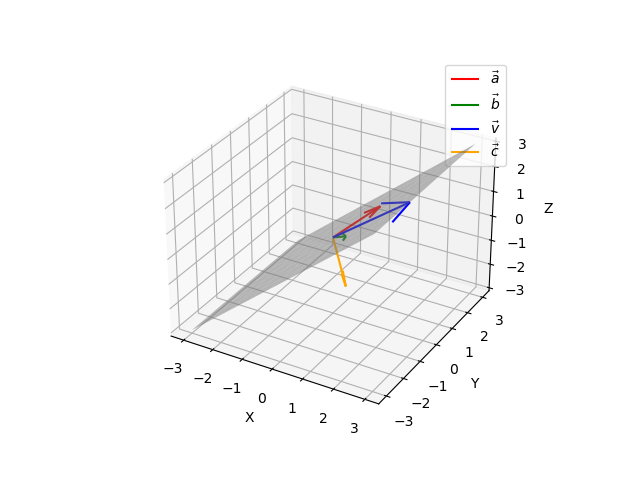
\includegraphics[width=1\columnwidth]{Figs/plot(py).png}
\end{figure}

\end{document}
